\documentclass[12pt,oneside]{uhthesis}
\usepackage{subfigure}
\usepackage[ruled,lined,linesnumbered,titlenumbered,algochapter,spanish,onelanguage]{algorithm2e}
\usepackage{svg}
\usepackage{amsmath}
\usepackage{amssymb}
\usepackage{amsbsy}
\usepackage{caption,booktabs}
\captionsetup{ justification = centering }
%\usepackage{mathpazo}
\usepackage{float}
\setlength{\marginparwidth}{2cm}
\usepackage{todonotes}
\usepackage{listings}
\usepackage{xcolor}
\usepackage{multicol}
\usepackage{graphicx}
\usepackage{multirow}

\graphicspath{{Graphics/}}

\floatstyle{plaintop}
\restylefloat{table}
\addbibresource{Bibliography.bib}
% \setlength{\parskip}{\baselineskip}%
\renewcommand{\tablename}{Tabla}
\renewcommand{\listalgorithmcfname}{Índice de Algoritmos}
%\dontprintsemicolon
\SetAlgoNoEnd

\definecolor{codegreen}{rgb}{0,0.6,0}
\definecolor{codegray}{rgb}{0.5,0.5,0.5}
\definecolor{codepurple}{rgb}{0.58,0,0.82}
\definecolor{backcolour}{rgb}{0.95,0.95,0.92}

\lstdefinestyle{mystyle}{
    backgroundcolor=\color{backcolour},   
    commentstyle=\color{codegreen},
    keywordstyle=\color{purple},
    numberstyle=\tiny\color{codegray},
    stringstyle=\color{codepurple},
    basicstyle=\ttfamily\footnotesize,
    breakatwhitespace=false,         
    breaklines=true,                 
    captionpos=b,                    
    keepspaces=true,                 
    numbers=left,                    
    numbersep=5pt,                  
    showspaces=false,                
    showstringspaces=false,
    showtabs=false,                  
    tabsize=4
}

\lstset{style=mystyle}

\title{Propuesta de sistema para la generación de reportes de enfrentamientos deportivos independiente de la fuente de datos}
\author{\\\vspace{0.25cm}Abel Molina Sánchez}
\advisor{\\\vspace{0.25cm}Dr. Yudivián Almeida Cruz\\\vspace{0.2cm}Lic. Manuel Santiago Fernández Arias}
\degree{Licenciado en Ciencia de la Computación}
\faculty{Facultad de Matemática y Computación}
\date{Fecha\\\vspace{0.25cm}\href{https://github.com/abel1927/Thesis}{github.com/abel1927/Thesis}}
\logo{Graphics/uhlogo}
\makenomenclature

\renewcommand{\vec}[1]{\boldsymbol{#1}}
\newcommand{\diff}[1]{\ensuremath{\mathrm{d}#1}}
\newcommand{\me}[1]{\mathrm{e}^{#1}}
\newcommand{\pf}{\mathfrak{p}}
\newcommand{\qf}{\mathfrak{q}}
%\newcommand{\kf}{\mathfrak{k}}
\newcommand{\kt}{\mathtt{k}}
\newcommand{\mf}{\mathfrak{m}}
\newcommand{\hf}{\mathfrak{h}}
\newcommand{\fac}{\mathrm{fac}}
\newcommand{\maxx}[1]{\max\left\{ #1 \right\} }
\newcommand{\minn}[1]{\min\left\{ #1 \right\} }
\newcommand{\lldpcf}{1.25}
\newcommand{\nnorm}[1]{\left\lvert #1 \right\rvert }
\renewcommand{\lstlistingname}{Ejemplo de código}
\renewcommand{\lstlistlistingname}{Ejemplos de código}

\begin{document}

\frontmatter
\maketitle

\begin{dedication}
    A mis padres.
\end{dedication}
\begin{acknowledgements}
    Quiero agradecer en primer lugar a mis padres, que han sido un ancla en todos los momentos de dificultad. Una 
bioquímica y un telecomunicador pueden revisar trabajos de cibernética, aunque solo sea la ortografía mamá. 
Un agradecimiento especial a mi Faby, por aguantar todos los momentos duros, por ser una inspiración, tu eres mi 
ejemplo de que siempre hay que seguir por mal dadas que vengan. Agradecimiento inmenso a mi abuela, siempre en función 
de que trabaje en la mayor calma posible. A mi hermano, por despertarme todos los días a las seis de la mañana, puedes 
estar seguro de que otro año hubieras ido caminando al servicio. Agradecer a mis hermanos de la vida, Ale, David, 
con ustedes al lado no hay moral que caiga. David, los apagones de tesis en el Naútico ya no nos los quita nadie, 
para la historia quedan. A los amigos que me regaló esta facultad, Ana, Javier, agradecerles las mañanas, tardes, 
noches, madrugadas compartidas, entre gente linda todo fluye mejor. Agradecer a todos mis amigos, familiares y profesores 
que han formado parte de este camino, me es imposible mencionarlos a todos, los llevo conmigo.
Agradecer a mis tutores Yudivián Almeida y Manuel Santiago por su guía y su disposición en todo momento.
\end{acknowledgements}
\begin{opinion}
    
    El estudiante Abel Molina Sánchez desarrolló satisfactoriamente el trabajo de diploma 
titulado “Generación automática de reportes textuales sobre enfrentamientos deportivos”. En este 
trabajo el estudiante propuso el diseño de un sistema para la generación automática de notas 
textuales sobre eventos deportivos. La idea general seguida fue la definición de un esquema general, 
o meta-esquema, de tuplas (4-tuplas) de conocimiento sobre las cuales se pudieran implementar, 
siguiendo una metodología genérica, funciones de realización particulares. 
    
    Para validar esta propuesta, el estudiante propuso esquemas particulares para dos deportes con 
características diferentes: el fútbol y el boxeo. Además, propuso un conjunto de funciones de 
realización lingüística para cada caso. Con ello pudo mostrar como se generaban distintos reportes 
para bases de conocimiento diferentes y así mostrar la validez y factibilidad de la propuesta.
    
    Para poder afrontar el trabajo, el estudiante tuvo que revisar literatura científica relacionada 
con la temática así como soluciones existentes y bibliotecas de software que pueden ser apropiadas 
para su utilización. Todo ello con sentido crítico, determinando las mejores aproximaciones y también 
las dificultades que presentan.
    
    Todo el trabajo fue realizado por el estudiante con una elevada constancia, capacidad de trabajo y 
habilidades, tanto de gestión, como de desarrollo y de investigación. 
    
    Por estas razones pedimos que le sea otorgada al estudiante Abel Molina Sánchez la máxima calificación 
y, de esta manera, pueda obtener el título de Licenciado en Ciencia de la Computación.
    
    
Dr. Yudivián Almeida Cruz

\end{opinion}
\begin{resumen}
	La Generación de Lenguaje Natural, como subcampo de la Inteligencia Artificial y la lingüística computacional, ha despertado cada vez mayor interés por su impacto en la 
automatización de la generación de texto en distintos escenarios. Son varios los sistemas que buscan producir textos a partir de datos en el área del deporte. Aun así, 
no abundan los sistemas desarrollados en idioma español y que sean independientes de la fuente de los datos. En el presente trabajo de tesis se propone un diseño de sistema 
para la generación automática de resúmenes de enfrentamientos deportivos independiente de la fuente de datos. Se propone un esquema general para definir las entradas 
específicas por deporte siguiendo una estructura de tuplas de conocimiento. Se presenta una propuesta de diseño para los modelos específicos de los deportes. La propuesta se valida 
a través de la implementación de un sistema que genera resúmenes de partidos de fútbol y combates de boxeo. Los modelos de generación siguen el estándar basado en reglas y plantillas.
\end{resumen}

\begin{abstract}
	Natural Language Generation, as a subfield of Artificial Intelligence and computational linguistics, has aroused increasing interest due to its impact on the automation of text 
generation in different scenarios. There are several systems that seek to produce texts from data in the area of sport. Even so, there are not many systems developed in Spanish and 
that are independent of the source of the data. In this thesis work, a system design is proposed for the automatic generation of summaries of sports matches independent of the data 
source. A general scheme is proposed to define the specific entries by sport following a structure of knowledge tuples. A design proposal for specific sports models is presented. The 
proposal is validated through the implementation of a system that generates summaries of soccer matches and boxing matches. The generation models follow the standard based on rules and 
templates.
\end{abstract}
\tableofcontents
\listoffigures
% \listoftables
% \listofalgorithms
%\lstlistoflistings

\mainmatter

\chapter*{Introducción}\label{chapter:introduction}
\addcontentsline{toc}{chapter}{Introducción}

    Desde hace varios años la Inteligencia Artificial (IA) viene revolucionando e \\impactando significativamente en muchas esferas de la 
vida del hombre. Dentro de la IA uno de los campos que más actividad tiene es el Procesamiento de Lenguaje Natural (PLN). Este abarca el conjunto de 
t\'ecnicas computacionales que tienen como objetivo el trabajo con el lenguaje humano, que van desde la extracci\'on de entidades en textos hasta modelos 
de comprensi\'on y generación de textos. Tanto la generación de texto a texto (\emph{text-to-text}, en inglés) como la generación de 
datos a texto (D2T por sus siglas en inglés, \emph{data-to-text} ) son instancias de la Generación de Lenguaje Natural (GLN). Reiter y Dale \brackcite{Reiter1997BuildingAN} 
caracterizan la GLN como el subcampo de la IA y la lingüística computacional que se ocupa de la construcción de sistemas informáticos que pueden 
producir textos comprensibles a partir de alguna representación no lingüística subyacente de la información. 
Esta definición se adapta fácilmente a los sistemas cuya entrada consiste en datos y es asumida en este trabajo para referirse a los sistemas de GLN. 
    
    
    Existe consenso en la forma en que la salida de un sistema de GLN debe presentarse: texto. Sin embargo, no hay establecido un est\'andar en cuanto a la forma en 
que se presentan los datos para su procesamiento, variando de un sistema a otro \brackcite{reiter_dale_2000,Gatt2018SurveyOT}. Como regla general el texto producido por estos sistemas 
debe mantener fidelidad a los datos que lo originan y debe ser consecuente con su intención comunicativa \brackcite{reiter_dale_2000}, no siendo lo mismo un 
sistema para la generación de diálogos que uno que tiene como objetivo describir resúmenes biográficos. Propuestas tempranas de sistemas como Ana \brackcite{kukich1983design} para 
generar reportes financieros, o como FoG \brackcite{goldberg1994using}, generador de reportes climáticos, comenzaron a mostrar las capacidades de estos 
modelos a la hora de dotar de interpretabilidad y relevancia datos que se presentaban de forma repetitiva y tediosa.
  
    En un contexto donde la producción de datos se ha acelerado como resultado de los avances tecnológicos y la digitalización de los sistemas industriales, se ha hecho necesario para 
las empresas el manejo y la interpretación de los mismos. Por esa raz\'on, algunas empresas se han especializado y han comenzado a brindar estos servicios a otras \brackcite{dale2020natural}. 
Un ejemplo es la compañía \textit{Automated Insights\footnote[1]{https://automatedinsights.com/}} que ha enfocado su negocio en brindar soluciones a otras corporaciones con vista a automatizar sus 
procesos de producción de texto. Entre los casos de uso clásico de estas soluciones encontramos, en el marco del comercio electr\'onico, la generación de descripciones de 
productos a partir de sus fichas técnicas. El periodismo ha sido otra de las esferas beneficiadas de estos avances en la GLN. La generación automática de noticias (conocida como 
periodismo robótico) está cada vez más extendida, al punto de que importantes editoriales como \textit{The Washington Post} han creado sus propios sistemas para la generación de 
texto a partir de datos\footnote[2]{https://www.washingtonpost.com/pr/wp/2017/09/01/the-washington-post-leverages-heliograf-to-cover-high-school-football/}. 
En este caso, su sistema se apoda \textit{Heliograf} y les permite cubrir todos los partidos de fútbol americano de las escuelas secundarias del área de Washington DC 
cada semana.

       \textbf{Problema}\\

    Aún con el desarrollo de los sistemas de GLN y su mayor asimilación en diversos ámbitos, siguen siendo absolutamente predominantes los 
sistemas que tienen el inglés como idioma de referencia a la hora de generar el texto de salida. En la literatura consultada no abundan las soluciones 
en lenguaje español en este campo, entre otras razones influenciado por la mayor complejidad estructural del español como lenguaje, así como el menor número 
de herramientas específicas para éste. De la misma forma ésto impacta directamente en los sistemas que tienen como objetivo comunicativo los eventos deportivos. Siendo el deporte un objeto de mucho interés en la 
comunidad hispanohablante en general y en Cuba en particular, se hace necesario ampliar los escenarios existentes desde esta perspectiva.

    Los sistemas analizados en la literatura consultada en su mayoría se basan en un conocimiento explícito del dominio a tratar así como en una 
estructuración predefinida de los datos en base al dominio. A su vez, son muchas las propuestas que parten de la obtención de los datos desde 
la fuente como parte propia del sistema y no propiciados por el usuario. Son pocos los sistemas funcionales, fuera de la industria, capaces de 
desacoplarse de las fuentes de datos y de abarcar desde una misma estructura distintos dominios.\\

    %Los modelos neuronales están impactando el estado del arte de muchas tareas en el campo del PLN. Se hace necesario 
%acercar el prisma hacia los mismos desde el punto de vista de la GLN.\\

   \textbf{Motivaciones}\\

    A partir del problema existente y las perspectivas que se abren en el campo de la GLN, surge la motivación del presente trabajo. Siendo el deporte un campo 
que despierta tanto interés y que es fuente de entretenimiento de muchas personas, sentar las bases del diseño de un sistema para la generación de resúmenes en español de 
eventos deportivos es un reto estimulante. Por su carácter estadístico y su gran audiencia, el deporte es una de las esferas que se puede beneficiar claramente del desarrollo de los sistemas 
de generación automática de texto. Muchos trabajos se han enfocado en este tema \brackcite{theune2001data, van2017pass, gunasiri2021automated}. Y aunque es relativamente sencillo encontrar en la web 
los datos o tablas estadísticas de un determinado enfrentamiento deportivo, la gran variedad de eventos que se suceden constantemente hacen 
que sea humanamente imposible darle cobertura a cada uno de ellos a nivel de narración y resumen. Por esta razón es motivante desarrollar  sistemas que sean capaces de cubrir muchas esferas del deporte.\\
Asímismo este trabajo se presenta en el marco de las líneas de investigación existentes en el 
grupo de Inteligencia Artificial de la Facultad de Matemática y Computación de la Universidad de La Habana (MATCOM) y puede servir de base para futuros trabajos que sigan ampliando y profundizando en la GLN.\\


    \textbf{Antecedente}\\

    La intención de adentrarse en la investigación de los sitemas de GLN dentro del departamento de IA de MATCOM comenzó con la propuesta, en 2019, 
de realizar un modelo GLN capaz de dar cobertura a las actuaciones destacadas de los peloteros cubanos en las Grandes Ligas de Béisbol. La misma derivó 
en el trabajo de tesis de Roberto Balboa González \brackcite{balboa2020}. Este primer acercamiento a la GLN sirvió para buscar nuevos escenarios a abarcar 
desde el punto de vista de esta disciplina. %El resto de los antecedentes vienen enmarcados en el estudio de la literatura y de los sistemas existentes dentro del campo de la GLN que 
%se presentan en un capítulo posterior.%

A pesar de los avances indiscutibles en el campo de la GLN queda aún mucho por hacer. Se considera que es interesante ampliar los sistemas que den cobertura informativa a los eventos 
deportivos en idioma español. Además, es motivante crear un diseño de sistema para la generación de resúmenes textuales de enfrentamientos deportivos, que pueda servir dentro del 
grupo de IA de MATCOM como antesala de futuras investigaciones y aplicaciones.


Teniendo en cuenta estos antecedentes, y partiendo de la hipótesis de que es posible definir un esquema general para representar los datos que describen los enfrentamientos deportivos,
se arriba al objetivo del presente trabajo.\\

%se presenta un prototipo de sistema capaz de generar resúmenes de eventos deportivos a partir de los datos prove\'idos por 
%el usuario. Se utiliza el futbol y el boxeo como muestras para validar la propuesta. 

    %Un sistema de este tipo tiene diversos casos de uso, y entre otros, sirve para describir eventos de interés para un 
%determinado público que pudieran quedar fuera de la cobertura noticiosa de los medios de prensa. En cualquier otro escenario, 
%su utilidad queda marcada por las necesidades que quieran cubrir sus usuarios, con la única condición de poseer los datos.

    \textbf{Objetivo}\\

    Proponer el diseño de un sistema para la generación de res\'umenes o reportes de eventos deportivos 
independiente de la fuente de datos del dominio, utilizando como muestras para la validación el fútbol y el boxeo.
%A partir de dicho diseño se presentan dos modelos capaces de generar resúmenes de partidos de 
%fútbol y combates de boxeo. 


    Para la consecución del objetivo es necesario:

    \begin{itemize}
        %\item Estudiar la literatura relacionada con la GLN y determinar los enfoques factibles.
        \item Analizar el dominio y determinar características comunes y relevantes de los eventos deportivos.
        \item Crear un esquema general a partir del cual poder definir esquemas específicos para la entrada de datos de los distintos deportes.
        \item Diseñar un sistema para la generación de resúmenes.
        \item Validar la propuesta con dos modelos de generación de texto basados en reglas y plantillas para el fútbol y el boxeo.   
    \end{itemize}

    %\begin{itemize}
    %    \item Estudiar la literatura relacionada con la GLN y determinar los enfoques factibles. 
    %    \item Comprobar los sistemas de generación relacionados con el dominio (eventos deportivos) y sus caracter\'isticas.
    %    \item Estudiar el dominio, y determinar los rasgos distintivos y comunes entre los eventos deportivos.
    %    \item Diseñar un esquema de eventos comunes característicos entre los deportes que de lugar a un esquema específico de cada uno.
    %    \item Plantear una estructura intermedia para el ingreso de los datos en base al esquema general diseñado. 
    %    \item Diseñar e implementar los modelos generadores de texto.
    %    \item Presentar el sistema funcional para la generación de resúmenes.       
    %\end{itemize}

    \textbf{Estructura del trabajo}\\

    El resto del trabajo se organiza de la siguiente manera. El capítulo 1 aborda los problemas generales de los sistemas de GLN 
y las distinas técnicas relevantes en la literatura para su solución. En el capítulo 2 se presenta la propuesta de meta esquema para la 
representación de los datos de entrada y la metodología para definir los esquemas específicos. En el capítulo 4 se presenta la validación
de la propuesta a través del resultado de los modelos generadores para el fútbol y el boxeo. Mientras 
en el capítulo 4 se analizan los detalles de la implementación. El trabajo concluye con la presentación de las 
conclusiones y recomendaciones.
\chapter{Estado del Arte}\label{chapter:state-of-the-art}


    Los sistemas de NLG normalmente reciben los datos de forma estructurada, pero esta estructura puede variar de un sistemas a otro.
La natualeza de los datos es diferente con lo cual sus representaciones pueden ir desde rergistros de base de datos, bases de conocimiento, 
grafos de conocimiento, o estructuras intermedias que utilizan representaciones del tipo clave-valor como pudiera ser el formato JSON, entre otras. 
Por ejemplo, en (~\cite{Yu2006ChoosingTC}) obtienen los datos en forma de series temporales, mientras que en (~\cite{kukich1983design}) los trabajan a 
partir de una base de datos de registros financieros.

En cuanto a la arquitectura, el diseño de sistemas NLG es un campo abierto donde no existe un amplio consenso. Existe una diversidad de propuestas e implementaciones 
que varían en dependencia del desarrollador y del problema para el cual se crea el sistema NLG. En este sentido, es difícil identificar elementos comunes y proporcionar una abstracción 
completa que sea aplicable a la mayoría de los sistemas NLG (~\cite{ramos2016role}).


 Sin embargo, la arquitectura propuesta por Riter y Dale en (~\cite{Reiter1997BuildingAN}) se ha tomado como el estandar de facto 
dentro de este campo, lo que no implica que muchos sistemas no plantearan estructuras diferentes (~\cite{Perera2017RecentAI}). 
Esta arquitectura de tubería (\emph{pipeline} en inglés), o modular, establece que los sistemas NLG pueden dividirse en módulos 
que encapsulen distintas tareas dentro del proceso de generación del texto.

    

    \begin{figure}[!]
        \begin{center}
            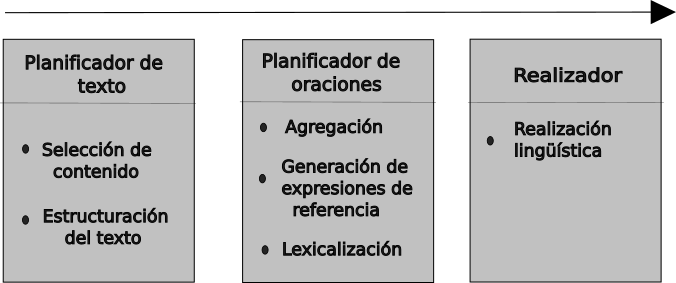
\includegraphics[width=\textwidth]{Graphics/arquitecturaPipeline_Capa 1.png}
        \end{center}
        \caption{Arquitectura modular planteada en (~\cite{Reiter1997BuildingAN}).}
        \label{fig_arq_Pipeline}
    \end{figure}


\section{Tareas principales de los sistemas Generación de Lenguaje Natural}

    Hasta hoy considerado como el punto de referencia y texto más completo en el campo de GLN(\cite{Gatt2018SurveyOT}), el libro de Ehud Riter y
Robert Dale: Building Natural Language Generation Systems(~\cite{reiter_dale_2000}), sienta las bases y define las que se han asumido como tareas principales 
de un sistema de GLN:

\begin{itemize}
    \item Determinación del contenido: decidir qué información es relevante.
    \item Estructuración del texto: determinar en qué orden se presentará la información.
    \item Agregación: decidir qué información se presenta en cada oración.
    \item Lexicalización: encontrar las palabras y frases adecuadas para expresar información.
    \item Generación de expresiones de referencia: selección de las palabras y frases para identificar entidades del dominio.
    \item Realización lingüística: conformación del texto con oraciones bien formadas.
\end{itemize}


Estas tareas naturalmente se puden dividir entre las que envuelven el proceso de elegir qué decir y de qué forma (planificación del contenido) 
a aprtir de los datos, y las que tienen un caracter más orientado al proceso lingüístico de elegir las términos adecuados para la expresión 
en si( realización)( ~\cite{Gatt2018SurveyOT}). Cada una de estas tareas, aunque no presentes todas en todos los sitemas,  presentan distintos 
objetivos dentro de los mismos y existen distintas técnias para cada una de ellas en la literatura.
    
\subsection{Determinación del contenido}

    Cada sistema GLN tiene un objetivo comunicativo, lo cual hace necesario determinar que información del dominio es relevante y debe 
estar representada en el texto final(\cite{reiter_dale_2000}). Los sistemas pueden presentar una especificación de los datos de la entrada 
o seleccionar un subconunto de los mismos(\cite{reiter_dale_2000}).

    El reconocimiento de patrones es una de las t\'ecnicas utilizadas con este fin.  SumTime-Turbine(~\cite{Yu2006ChoosingTC}) es un sistema funcional para crear
 informes sobre un mecanismo de turbinas de gas. En un contexto donde la cantidad de datos en muy grande y en su mayoría irrelevante, 
 los autores con ayuda de los expertos del dominio crean un modelo que permite reconocer patrones en los datos así como luego, utilizando una base de datos de patrones 
antiguos determinar los patrones relevantes a ser expresados en el informe. 

    Existen muchos sistemas de GLN que utilizan modelos basados en reglas como \'unica metodolog\'ia para la selecci\'on de contenido(~\cite{reiter_dale_2000,Perera2017RecentAI}). Bouayad-Agha, Casamayor y 
Wanner (~\cite{BouayadAgha2011ContentSF}) en su trabajo presentaron el dise\~no te\'orico de un sistema para generar resumenes de partidos de 
futbol de la Liga Espa\~nola. Para la conformaci\'on del mismo describieron la construcci\'on de una garn base de conociminetos del dominio as\'i como 
un estricto sistema de reglas para la selecci\'on de contenido. Es relevante este enfoque ya que con un conocimiento del dominio a tratar y de la intenci\'on comunicativa del texto a producir 
es posible implementar reglas que den lugar a la selección del contenido relevante(~\cite{Reiter1997BuildingAN,reiter_dale_2000}). 

    Como el proceso de creaci\'on de reglas puede ser tedioso y es dependiente del dominio(~\cite{Reiter1997BuildingAN}) aparecieron iniciativas que para la automatizaci\'on de esta tarea. Un enfoque 
basado en t\'ecnicas de aprendizaje autom\'atico es el presentado por Dubou\'e y McKeown(~\cite{Dubou2003StatisticalAO}). En este trabajo plantearon un modelo de aprendizaje supervisado que a trav\'es de
un corpus de resultados deseados(texto escrito por humanos) aparejados con los tipos lingüísticos de la entrada(distintos tipos de datos que recibe el sistema) determina un conjunto de constantes. Estas constantes 
expresan si determinado dato de entrada debe aparecer o no reflejado en la salida y bajo que condiciones. Este sistema se utilizó para la generación de descripciones biográficos cortas que resumirán hechos 
importantes sobre personajes famosos.

\subsection{Estructuración del texto}

    La estructuración del texto o planificación del discurso es el proceso donde se da orden y estructura al conjunto de mensajes a expresar en el texto producido. En un texto la información se presenta en un orden particular 
y, por lo general, hay una estructura subyacente a la presentación. La complejidad de la estructura de los textos puede variar de un sistema a otro. Una buena estructuración puede hacer que un texto sea mucho más fácil 
de leer(~\cite{Reiter1997BuildingAN}).

    Los primeros enfoques para la estructuración de documento se basaron en reglas estructuradas hechas a mano dependientes del dominio(~\cite{Gatt2018SurveyOT}). A este enfoque se le conoce como el enfoque basado en esquemas, nombre que 
se deriv\'o del trabajo de Kathleen R. McKeown(~\cite{mckeown1985discourse}) cuando acu\~n\'o el t\'ermino \textit{"schematta"}. En la construcci\'on de su sitema TEXT(~\cite{mckeown1985discourse}), McKeown, luego del an\'alis de muchos 
ejemplos del dominio, concluyó que dado un objetivo comunicativo, la información tiende a transmitirse en el mismo orden. En base a esto defini\'o estructuras(esquemas) que determinan posibles combinaciones de atributos, formando patrones 
y plantillas. De esta forma el sistema, dada una intenci\'on comunicativa, puede seleccionar un esquema que defina la forma de transmitir la información. La mayor\'ia de los sitemas que siguen este enfoque utilizan 
las Matrices de Valores de Atributos(AVMs por sus siglas en inglés, Attribute Value Matrics)(~\cite{Perera2017RecentAI}).

    Las estructuras ret\'oicas son otro de los mecanismos que se utilizan para la planificación. Estas se derivan del trabajo de Mann y Thompson quienes introdujeron la Teor\'ia de la Estructura Ret\'orica(RST por
sus siglas en inglés, Rhetorical Structure Theory)(~\cite{mann1988rhetorical}). Las estructuras ret\'oricas constituyen un m\'etodo lingüístico para la descripci\'on de texto caracterizando las estructuras primarias del mismo y estableciendo 
relaciones funcionales entre sus distintas partes. La RST tiene como base los conceptos de n\'ucleo y sat\'elite que definen las partes del texto entre las que se estable un relaci\'on. Los distintos sistemas que utilizan las estructuras ret\'oricas 
para la estructuraci\'on del texto definen que tipo de relaciones establecen. Ejemplo de relaciones lingüísticas planteadas por Mann y Thompson en su trabajo son: motivaci\'on, causa, condici\'on, cirscuntancia, etc(~\cite{mann1988rhetorical}). 

\subsection{Agregación}

    En un texto, cada parte de información no tiene que estar presente en oraciones independientes. Hay escenarios donde es 
deseable que distintos mensajes sean transmitidos en una misma oraci\'on. La agreagaci\'on puede permitir crear texto de mayor 
calidad o eliminar repeticiones inncesarias que vayan en contra de la fluidez del texto(\cite{Gatt2018SurveyOT}).
    Un ejemplo de agregaci\'on, en el dominio del f\'utbol, describiendo el hecho de dos anotaciones consecutivas de un jugador, puediera ser:

\begin{itemize}
    \item (1) Ronaldo anot\'o para el Real Madrid en el minuto 2. Ronaldo anot\'o para el Real Madrid en el minuto 8.
    \item (2) Ronaldo anot\'o dos veces para el Real Madrid antes del minuto 8.
\end{itemize}

    En (2) se evita la repetici\'on y la información se presenta de forma m\'as fluida y natural al lector.
    
    Reape y Mellish(~\cite{reape1999just}) realizaron un estudio sobre la tarea de agregación dentro de los sitemas de generación 
de texto, distinguiendo entre la agregación a nivel semántico(más dependiente del dominio) y a nivel sintáctico. Muchos de los primeros 
trabajos sobre agregación fueron dependientes del dominio, centrados en la aplicación de reglas(por ejemplo, 
"si un jugador marca dos goles consecutivos, expr\'esalo en la misma frase') generalmente hechas a mano(ejemplo ~\cite{Shaw1998ClauseAU}). 
Con el tiempo aparecieron propuestas que utilizan enfoques de aprendizaje autom\'atico. SPoT es un sistema que se present\'o en ~\cite{walker2001spot}) 
contituendo uno de los primeros sistemas entrenados que incluye la tarea de agregación. Los autores plantearon una metodolog\'ia basada en la producci\'on 
de varios textos para una misma entidad informativa utilizando diferentes cl\'ausulas de agregación asociadas al dominio. Despu\'es utilizaron un modelo 
entrenado para dar un valor a cada una de las salidas estableciendo un ranking a partir del cual hacer la selección. Mientras, Barzilay y Lapata(~\cite{Barzilay2006AggregationVS})
plantearon el problema en términos de optimización global. Realizan una clasificación inicial sobre pares de entradas de la base de datos que determina 
si deben agregarse o no en función de su similitud por pares. Posteriormente, seleccionan un conjunto globalmente óptimo de entradas relacionadas en función
de un grupo de restricciones.

    Con la agregación sintáctica, podría decirse que es más factible definir reglas independientes del dominio para eliminar la 
redundancia(~\cite{Gatt2018SurveyOT}). Por ejemplo, convertir (3) en (4) a continuación

\begin{itemize}
    \item (3) Ronaldo marcó en el minuto 2 y marcó de nuevo en el minuto 8.
    \item (4) Ronaldo marcó en el minuto 2 y de nuevo en el 8.
\end{itemize}
    
podría lograrse identificando las frases verbales paralelas en las dos oraciones conjuntas y eliminando el sujeto y el verbo en la segunda.

\subsection{Lexicalización}

    La lexicalización es un proceso muy importante dentro de un sitema de GLN. Es el proceso durante el cual se 
seleccionan la palabra o palabras que expresan un concepto o relaci\'on(~\cite{Reiter1997BuildingAN}). Una de las 
complicaciones del proceso de lexicalización est\'a dada porque una misma relación puede ser expresada de 
distintas formas. Por ejemplo, el evento de la anotación de un gol en un partido de fútbol puede ser expresado como:
¨marcar un gol¨, ¨poner el balón en la red¨, ¨conseguir una anotación¨. La complejidad de este proceso depende en gran 
medida del número de alternativas que el sistema pueda o quiera contemplar. Las restricciones contextuales también juegan 
un papel importante a la hora de expresar un mensaje, por ejemplo, la expresion ¨marcó un gol¨ es desafortunada si el evento 
descrito es un gol en propia puerta(~\cite{Gatt2018SurveyOT}).

    El proceoso de lexicalización puede seguir dos vertientes principales. Una ser\'ia la realizaci\'on de la  
lexicalización de la forma m\'as simple posible, lo cual se lleva a cabo generalemente utilizando t\'ecnicas para el llenado de 
plantillas lexicalizadas. De otra forma se puede realizar este proceso en mayor profundidad utilizando t\'ecnicas m\'as complejas  
que permmitan por ejemplo: la eliminaci\'on de palabras innecesarias, la selección de vacablos que maximicen la efectividad del obetivo 
comunicativo del texto, la uni\'on de t\'erminos que se aparejan frecuentemente en el dominio(~\cite{Perera2017RecentAI}).

    Los enfoques basados en reglas son de los m\'as utilizados, pudiedo variar en complejidad entre un sistema y otro. \textit{EasyText}(~\cite{danlos2011easytext}) 
es un ejemplo de sistema que utiliza reglas para la lexicalización pero que da un paso m\'as all\'a ya que consume de una base de datos 
l\'exica creada principalmente por lingüístas. Esta alternativa permite una lexicalización m\'as avanzada pero a su vez es altamente 
costosa en recursos.

    La utilizaci\'on de ontolog\'ias tambi\'en est\'a presente en este proceso de los sistemas de GLN. El uso de ontologías permite 
al sistema ganar en adaptabilidad ya que encontrar una ontología para un dominio determinado es más sencillo que encontrar un corpues para 
el mismo. Así mismo ofrecen una mayor cobertura de las representaciones semánticas que los corpus(~\cite{Perera2017RecentAI}). En ~\cite{cimiano2013exploiting} introducen 
un modelo que utiliza este enfoque presentado en el dominio de las recetas de cocina.


\subsection{Expresiones de referencia}

    Robert Dale y Ehud Rither describieron la generación de expresiones de referencias dentro de un sitema de GLN como la tarea de 
indentificar la expresión, comprensible de cara al usuario, a utilizar para indetificar a una instancia del dominio(~\cite{reiter_dale_2000,Gatt2018SurveyOT}). 
Los primeros m\'etodos para la selección de referencias fueron los algoritmos generativos que en común presentan la necesidad de tener conocimiento 
contextual y de propiedades de las entidades(~\cite{Gatt2018SurveyOT}). De este orden es el algoritmo incremental cuya base se plant\'o en ~\cite{dale1995computational}. 
El algoritmo, en base a conocer la entidad a referenciar(objetivo), el resto de entidades(llamadas distractores) y el grupo de propiedades que definen entidandes en el dominio,
busca determinar un conjunto de propiedades \'unicas que definan al objetivo y lo diferencien del resto.

    Muchos de los trabajos que versan sobre este tema hacen énfasis en un tipo determinado de referencia(~\cite{ferreira2018neuralreg}). La selección 
puede ser de un pronombre(\'el/ella), una descripci\'on( Sim\'on, el jugador cubano) o en la generación de nombres propios(Frederich Cepeda/Cepeda). 
Rither y Dale(~\cite{reiter_dale_2000}) plantean una diferencia entre una referencia temprana(primera vez que se menciona una 
entidad en el texto) y una tard\'ia(cuando se refiera a una entidad mencionada anteriormente). Plantearon el uso de los nombres propios a la hora 
de introducir una entidad, luego, en base a cla\'usulas seleccionar un pronombre apropiado, ejemplo:

\begin{verbatim}
    si el referente fue mencionado en la oración anterior;
    entonces utiliza un pronombre
\end{verbatim}

a su vez es necesario considerar los escenarios donde la generaci\'on de expresiones de referencia pudiera llevar a ambigüedades:

\begin{itemize}
    \item Benzema anotó dos para el Real Madrid mientras Luka Modric brindó dos asistencias. Él fue elegido el jugador del partido... 
\end{itemize}

    En \cite{siddharthan2011information} los autores realizaron un estudio emp\'irico del comportamiento de las referencias hacia parsonas basadas en 
su nombre propio en el contexto de los art\'iculos de noticias. Para ello utilizaron un corpus de noticias en inglés de diferentes agencias de prensa y 
cuantificaron las diferentes formas de referencia seg\'un el momento referencial de la instancia(temprana o tard\'ia). Como resultado de este trabajo 
arrojaron que el nombre completo de la entidad suele utilizarse como primera referencia en la pr\'actica totalidad de los casos mientras que en su mayor\'ia
el apellido se utiliza cuando se trata de una referencia tard\'ia. 

   %Entre las propuestas recientes para la generaci\'on de entidades referenciales encontramos la presentada en \cite{ferreira2018neuralreg}. Los autores presentan 
%\textit{NeuralREG}, un modelo de aprendizaje profundo implementado como multi-encoder, attention-decoder con biderectional LSTM(Long-Short Term Memory). Para el 
%entrenamiento del modelo utilizaron una versi\'on deslexicalizada del corpus \textit{WebNLG} . Cada entidad presente en los datos fue mapeada
% con diferentes etiquetas de forma tal que 

\subsection{Realización lingüística}

    El proceso de realizaci\'on lingüística es el que da lugar a la formaci\'on final del texto expresado en oraciones con una 
estructura gramatical correcta y coherente con el mensaje a transmitir. Esta tarea implica ordenar los constituyentes de una oración, 
así como generar las formas morfológicas correctas (incluidas las conjugaciones y la concordancia de los verbos). A menudo, los 
realizadores también necesitan insertar palabras funcionales (como verbos auxiliares y preposiciones) y signos de puntuación(~\cite{Gatt2018SurveyOT}).
   
    Una de las t\'ecnicas m\'as utilizadas es la que incluye el uso de plantillas predefinidas para expresar mensajes(\cite{Gatt2018SurveyOT}). Las 
plantillas, aunque requieren una carga intensiva de trabajo para lograr mayor variabilidad en el texto a producir permiten un control total sobre 
la calidad y la correctitud del texto a elaborar. Un ejemplo de plantilla:

\begin{verbatim}
    $equipo_1 venció $pts_equipo_1 a $pts_equipo_2 a $equipo_2
\end{verbatim}

    Dicha plantilla, que representa el resultado de un enfrentamiento entre dos equipos se completa con la información extraida de los datos y a la hora de 
la realización el resultado pudiera ser el siguiente:

\begin{verbatim}
    Industriales venció 10 a 1 a Granma
\end{verbatim}

\section{Propuestas neuronales para la generación de texto}
    Al ingual que en otras áreas del procesamiento de lenguaje natural, el dominio de la GLN se ha visto 
impactado por el auge de las soluciones basadas en redes neuronales (~\cite{Gatt2018SurveyOT,sharma2022innovations}). 
Mientras los sistemas tradicionales de D2T siguen una estructura modular con etapas bien definidas (estructuración, relalización, etc), 
los modelos neuronales variaron el camino hacia estructuaras \emph{end-to-end} (de extremo a extremo, en español), unificando 
en muchas casos, varias tareas en un solo paso de entrenamiento.

    Los trabajos que siguieron este enfoque (~\cite{lebret-etal-2016-neural,mei2016talk,wiseman-etal-2017-challenges} ) plantearon modelos \emph{Seq2Seq} (de secuencia a secuencia, en español) que adoptan la 
influyente estructura de codificador-decodificador (~\cite{sutskever2014sequence}). Utilizan una red neuronal recurrente (RNN, \emph{Recurrent Neural Network}, en inglés) 
para codificar la entrada de un vector de representación el cual sirve a su vez como entrada auxiliar de otra RNN que hace de decodificador y produce el texto, y no tienen módulos 
específicos para mejorar la calidad del resultado más allá de los mecanismos gen\'ericos de atención y copia (~\cite{bahdanau2014neural,gu2016incorporating}). La popularidad de los módelos 
\emph{end-to-end} se vió impulsada y a la vez creó la necesidad de contar con corpus de datos paralelos que permitieran evaluar la calidad de las propuestas. Estos conjuntos de datos tenían que 
tener la suficiente cantidad de instancias para poder entrenar modelos de estas características. RotoWire (~\cite{wiseman-etal-2017-challenges}) es un punto de referencia ampliamente utilizado, se construyó con cerca de 
cinco mil pares de datos estadísticos de partidos de baloncesto y su correspondiente resumen descriptivo escrito por profesionales. En ~\cite{puduppully2019data}, los autores introdujeron MLB, un nuevo corpus con aproximadamente 
25 mil instancias de estádisticas aparejadas con descripciones en este caso en el dominio del beisbol. Otros conjuntos de datos hechos a mano como E2E (~\cite{novikova2017e2e}) se han construido para analizar tareas espec\'ificas 
como la capacidad de realización lingüística.

        \begin{figure}[!]
            \begin{center}
                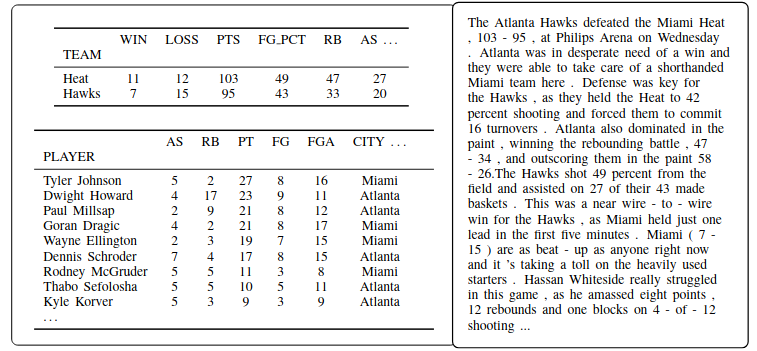
\includegraphics[width=\textwidth]{Graphics/rotowire_instancia.png}
            \end{center}
            \caption{Instancia de RotoWire (~\cite{wiseman-etal-2017-challenges}).}
            \label{fig_RotoWire}
        \end{figure}

 En ~\cite{wiseman-etal-2017-challenges} los autores mostraron la capacidad de estos modelos de producir un texto dotado de mayor 
fluidez en comparativa con propuestas tradicionales. A su vez, además de ser propensos a la alucinación (es decir, generan texto que no es compatible con la entrada), 
mostraron  deficiencias a la hora de seleccionar el contenido y/o estructurar el documento (por ejemplo, en el marco de una descripción biográfica, la omisión de la fecha de nacimiento es un relevante, 
mientras que de aparecer no es apropiado que lo haga en la última oración del escrito ). Para mejorar esta situación ~\cite{puduppully2019dataselandplan}  
presentaron una arquitectura que incorpora selección y planificación de contenido sin sacrificar el entrenamiento \emph{end-to-end}. Descompusieron la tarea de generación en dos etapas. Dado el corpus de 
registros de datos (junto con las descripciones), primero generaron un plan de contenido destacando qué información debía mencionarse y en qué orden para luego generar el documento teniendo en 
cuenta dicho plan. Un enfoque similar se planteó en ~\cite{chen2021neural}, mientras que en ~\cite{moryossef2019step}, desacoplaron por completo ambas fases, dejando solo el modelo neuronal para la realización del 
texto una vez desarrollada la estructura informativa.

        \begin{figure}[!]
            \begin{center}
                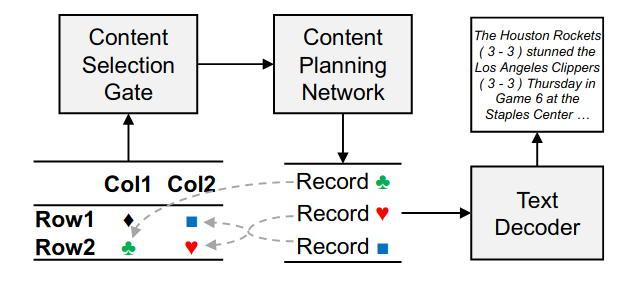
\includegraphics[scale=0.4]{Graphics/lapata_arquitectura.png}
            \end{center}
            \caption{Arquitectura del modelo presentado en ~\cite{puduppully2019dataselandplan}.}
            \label{fig_lapata_arquitectura}
        \end{figure}


    La utilización de modelos preentrenados en tareas de generación de texto-a-texto para producir texto a partir de datos en base al reentrenamiento 
fue de los enfoques que se exploraron recientemente. En (~\cite{kale2020text}) los autores utilizaron el modelo T5 (\emph{“Text-to-Text Transfer Transformer”}, su nombre en inglés) (~\cite{raffel2020exploring})
preentrenado para tareas de generación de resúmenes, traducción entre idiomas, clasificación de texto entre otras. Sus resultados fueron alentadores sobre todo desde el punto de vista de 
la generalizción. Este modelo, no solo tuvo una buena actuación en cuanto a la calidad del texto generado sino que también mostró buena adaptación a dominios distinos a los 
del reentrenamiento, lo cual constituyó una diferencia respecto a los modelos neuronales tratados anterioremente.


    Como quedó patente en (~\cite{wiseman-etal-2017-challenges,ferreira2019neural,duvsek2020evaluating,sharma2022innovations})  los sitemas basados en redes neuronales
 son capaces de producir texto que supera en fluidez y en evaluaciones humanas como la naturalidad a los sistemas tradicionales. Por contra, 
estos modelos siguen lidiando con su principal problema que es la presencia de alucinacinaciones en las salidas. Esta deficiencia es objeto de interés 
de los investigadores en este campo (~\cite{ji2022survey}). Por esta razón, Robert Dale, en su \textit{Natural language generation: The commercial state of
the art in 2020} (~\cite{dale2020natural}) planteó que estas soluciones, aunque prometedoras, se 
encuentran en fase principalmente académica y que en la industrian, en un entorno donde la fidelidad de los datos es crucial, su adopción general no ha llegado.   


\section{Sistemas para la generación de texto a partir de datos}

    Al referirse al campo de GLN, se puede afirmar que el mismo es ya un campo investigativo consolidado dada la cantidad 
de sistemas que han sido implementados y la variedad de los dominios de su aplicación práctica. FOG (\emph{Forecasting Generator}, en inglés) (~\cite{goldberg1994using}) es 
de los primeros sistemas funcionales para la generación de texto a partir de datos. Este, al igual que SumTime (~\cite{reiter2005choosing}) genera breves pronósticos del tiempo
a partir de los valores de variables meteórologicas. 

    En la escena industrial, propiciado por el desarrollo constante de herramientas para el análsis y captura de datos,
hubo empresas que detectaron en la generación de texto un nicho de mercado no cubierto y prometedor (~\cite{dale2020natural}). Compañías como \textit{Ax Semantic\footnote[1]{https://en.ax-semantics.com/}} y 
\textit{Narrativa\footnote[2]{https://www.narrativa.com/}} ofrecen soluciones para automatizar la descripción de productos para el comercio electrónico. 
\textit{Automated Insights} creó su plataforma para la generación de lenguaje natural, \textit{Wordsmith}. Este software da la posibilidad al usuario de crear un conjunto 
de plantillas basadas en reglas que desciben los datos que desea a tratar. A partir de las mismas, y en dependencia de su sofistición los textos generados pueden llegar a ser 
indistinguibles de los textos redactados por un humano. Precisamente en colaboración con \textit{Automated Insights}, la gran corporación de prensa \textit{Associated Press (AP)} generó l
las vistas previas de los partidos de una temporada regular de baloncesto, liberando a los periodistas de este trabajo. A su vez, \textit{Yahoo!} utiliza esta tecnología para crear informes 
de jugadores y resúmenes de partidos de fútbol del juego \textit{Fotball Manager} que es de gran interés para sus usuarios. Otro caso de uso dentro de la automatización de contenido en la prensa lo encontramos en \textit{PostData\footnote[3]{http://www.postdata.club/index.html}}, un sitio de periodismo 
de datos cubano, donde utilizan un modelo propio, \textit{ArmandBot} (~\cite{balboa2020}), para generar reportes sobre las actuaciones de los peloteros cubanos en grandes ligas.

    En la literatura hay propuestos varios modelos de sitemas para la GLN en el ámbito del deporte. Por ejemplo, en (~\cite{kanerva2019template}), apoyados en la constucción de un corpues de 2000 encuentros de hockey sobre hielo 
proponen un modelos de secuencia a secuencia, para generan narrativas sobre esta práctica deportiva. Hasan (~\cite{hasan2011automatic}) propuso un sistema basado en plantillas que sigue la arquitectura tradicional basada en módulos para 
modular para generar texto en inglés y bengalí\footnote[5]{El bengalí es el idioma nacional y el idioma oficial de la República Popular de Bangladesh} para generar resúmenes de juegos de críquet a partir de datos estructurados obtenidos de la web. 
Siguiendo el mismo enfoque, en ~\cite{gu2016incorporating} presentan otro sistema basado en plantillas para el críquet, en este caso al estilo propio de Sri Lanka.
 
En el caso del fútbol, una de las principales propuestas fue GoalGetter (~\cite{theune2001data}), un sistema de datos a voz en idioma neerlandés, que consta de dos módulos, uno para tranformar los datos en texto y 
otro para luego llevar el texto a sonido. GoalGetter tomó los datos de una página de Telexto que contenía los datos de uno o más partidos de fútbol. Una característica de este sistema es que propuso una arquitectura diferente al 
estándar modular de otros sistemas. En este caso, utilizó un solo módulo para la generación de texto que consumía una base de conocimiento con los nombres de los jugadores y equipos junto a un sistema de plantillas sintácticas.
 En base a este trabajo, en \cite{aires2016automatic} se propuso GameRecapper, un sistema capaz de generar resúmenes de partidos de fútbol de la liga portuguesa en idioma portugés. Este sistema obtenía los datos de \textit{www.zerozero.pt} 
una página web que contenía la información de partidos los partidos de cada jornada. Al módulo de generación agregaron a su vez una base de conocimiento y un conjunto de funciones léxico semánticas para mejorar la calidad del texto. De este trabajo es resaltó el hecho 
de que hicieron una caracterización más amplia del evento principal del fútbol, el gol, en su sistema de plantillas. Para cada distinto escenario propusieron la creación de plantillas oracionales específicas (primer gol del patido, último gol, gol que empata, etc).
Pass (~\cite{van2017pass}), es una propuesta basada en GoalGetter que busca diferenciar el texto producido en base a la audiencia del mismo. Para ellos establecen un sistemas de plantillas que abarca distintos posibles escenarios de resultado de un partido: victoria o derrota 
del equipo local, victoria o derrota del equipo visitante o empate. La elección de cual plantilla utilizar va en depencia de a qué afición irá dirigido el texto.  

    La gran mayoría de estos sistemas cuentan con un dominio específicos de aplicación, así como cuentan con una fuente de datos de la 
cual extraer la información a desarrollar. Por tanto, y aunque fuera posible la adaptabilidad, existe una depencia de la fuente de información. A su vez, el tener un dominio bien definido  
permite agreagar bases de conocimiento previo del mismo que enriquezcan los modelos. Predominan los sistemas basados en plantillas y reglas, variendo entre si su nivel de complejidad. Estos 
sistemas son especialmente adaptables y prácticos para idiomas distintos del inglés debido a que las herramientas de generación específicas desarrolladas son menores en compaaración (~\cite{gunasiri2021automated}). 
    En el presente trabajo se presenta un prototipo de sistema basado en la propuesta de un esquema general que permita definir esquemas específicos de entradas en formas de 4-tuplas (tuplas de cuatro elementos) de 
conocimiento de un deporte de enfrentamiento dos a dos ( beisbol, voleibol, judo, etc). A su vez, se seleccionan dos deportes, en este caso, futbol y boxeo, y a partir de las especifiaciones planteadas se 
se definen dos modelos capaces de generar un resumen informativo del evento en cuestión. Los modelos siguen el estandar basado en reglas plantillas simples de expresiones y oraciones.




    %\begin{figure}[!]
    %    \begin{center}
    %        \includegraphics[width=\textwidth]{Graphics/arquitecturatesisOk.png}
    %    \end{center}
    %    \caption{Arquitectura del modelo propuesto}
    %    \label{arquitecturadelmodelo2}
    %\end{figure}


 
    %\begin{figure}[htbp]
    %    \begin{center}
    %        %\includesvg{Graphics/arquitecturatesis3.svg}
    %        \includegraphics[width=\textwidth]{Graphics/arquitecturatesis3.svg}
    %    \end{center}
    %    \caption{Arquitectura del modelo propuesto}
    %    \label{arquitecturadelmodelo}
    %\end{figure}

    %\def\svgwidth{\textwidth}
            %\def\svgscale{1}

    %\begin{figure}[htbp]
    %    \centering
    %    \input{Graphics/arquitecturatesis6.pdf_tex} 
    %    \caption[]{Arquitectura del modelo utilizado}      
    %    \label{arquitecturadelmodelo}
    %\end{figure}

\chapter{Propuesta}\label{chapter:proposal}
 
    El objetivo de proponer el diseño de un sistema para generar resúmenes de eventos deportivos independiente de la fuente de datos 
planteó distintos retos. El primero de estos fue la necesidad de definir un esquema que permitiera abstraer las características 
generales del conjunto de deportes de enfrentamiento (enfrentamiento dos a dos). Junto con dicho esquema se necesitó 
definir una estructura común para la entrada de los datos que permitiera expresar los conocimientos del dominio. Se seleccionó 
una estructura basada en tuplas de cuatro elementos (cuatro-tuplas en lo adelante). A partir de esta estructura y en base 
al esquema de definición general se buscó poder determinar esquemas específicos para cada deporte que se fuera a incluir en el 
sistema. Cada uno de estos esquemas específicos son los que se encargan de definir un deporte de forma individual dentro del sistema.
Luego se realiza una propuesta general de diseño para concebir los modelos generadores de un deporte.
    
    En segunda instancia, se construye, en base a la propuesta, un esquema y su modelo correspondiente para generar 
resúmenes de partidos de fútbol. Lo mismo se realizó con un deporte de naturaleza diferente como el boxeo.

\section{Propuesta de Esquema General}

    Los deportes se pueden clasificar en la categoría de individuales o colectivos. En los deportes colectivos, las representaciones 
del enfrentamiento ocurren en base a equipos que agrupan a individuos. A su vez, en los deportes individuales son dos los contendientes.
Esta es la primera diferencia que se extrae en el análisis del conjunto de deportes. Las modalidades analizadas están representadas en \ref{tab:table_deportes_seleccionados}, 
clasificadas en individuales o colectivas.

% Please add the following required packages to your document preamble:
% \usepackage{multirow}
\begin{table}[]
    \begin{center}
    \begin{tabular}{|c|c|}
    \hline
    Colectivos                                                                                                                                          & Individuales                                                                                                     \\ \hline
    \multirow{5}{*}{\begin{tabular}[c]{@{}c@{}}Béisbol, Voleibol, \\ Fútbol, Tenis Dobles, \\ Baloncesto, Waterpolo, \\ Balonmano, Hockey\end{tabular}} & \multirow{5}{*}{\begin{tabular}[c]{@{}c@{}}Tenis, Esgrima, \\ Boxeo, Judo,\\ Lucha libre, Taekwondo\end{tabular}} \\
                                                                                                                                                        &                                                                                                                  \\
                                                                                                                                                        &                                                                                                                  \\
                                                                                                                                                        &                                                                                                                  \\
                                                                                                                                                        &                                                                                                                  \\ \hline
    \end{tabular}
    \caption{Deportes analizados}
    \label{tab:table_deportes_seleccionados}
    \end{center}
\end{table}

    De cada uno de estos deportes se analizó:

    \begin{itemize}
        \item Naturaleza de decisión: La mayoría de los deportes se definen como juegos 
        adversariales por acumulación de puntos. La entidad con mayor puntuación gana. Otros, como el tenis y el voleibol 
        se definen por cantidad de etapas ganadas (sets), y cada etapa se gana por puntos. A su vez, en el boxeo la definición 
        se deriva de votaciones de árbitros.
        \item Posibilidad de empate: Hay deportes como el fútbol en el que, según la competición o la fase de ésta, existe la posibilidad de 
        definirse sin ganadores ni perdedores.
        \item División de los eventos: La mayoría de los eventos se divide por etapas de tiempo.
        constante. Una excepción es el judo que ocurre de forma continua durante cuatro minutos. 
        \item Alargues de tiempo: La mayoría de los deportes, en caso de no definición en su tiempo reglamentario, presentan 
        etapas adicionales en forma punto de oro (ej. judo),  tiempos extras (ej. béisbol, fútbol), tiebreak (desempate, ej. voleibol, tenis).
        \item Roles: Dentro de los deportes los participantes ejercen roles, como puede ser su posición en los deportes colectivos. En los deportes 
        individuales estos roles no son tan explícitos.
        \item  Acciones principales: La definición de los eventos son las acciones relevantes que ocurren durante el tiempo de juego.
    \end{itemize}

    Del análisis también se extrajeron un conjunto de características que son comunes a los enfrentamientos deportivos: la sede, 
el público, la fecha. Asimismo, los enfrentamientos normalmente se encuadran dentro de un torneo, y existen distinciones entre categorías lo mismo sea 
de edad, sexo, u de otro tipo (ej. peso).

    A partir del análisis se definió un meta esquema general de tipos de entradas basado en una estructura de 
cuatro-tuplas de conocimiento.

\begin{table}[]
    \begin{center}

\begin{tabular}{|c|c|}
    \hline
    Tipo de Entrada  & Estructura                                                                                                               \\ \hline
    SEDE             & \begin{tabular}[c]{@{}c@{}}(TipoSEDE, \\ Nombre\\ Asistencia\\ Capacidad)\end{tabular}                                   \\ \hline
    TORNEO           & \begin{tabular}[c]{@{}c@{}}(TipoTORNEO\\  Nombre\\ Expresión de Género\\  Expresión de Categoría)\end{tabular}           \\ \hline
    ENFRENTAMIENTO   & \begin{tabular}[c]{@{}c@{}}(TipoENFRENTAMIENTO\\ Entidad\_1\\  Entidad\_2\\  Expresión de Fecha)\end{tabular}            \\ \hline
    ROLENJUEGO       & \begin{tabular}[c]{@{}c@{}}(TipoROLENJUEGO\\  Entidad del Rol\\  Entidad Complementaria\\ Rol Complementario)\end{tabular}   \\ \hline
    RESULTADOPARCIAL & \begin{tabular}[c]{@{}c@{}}(TipoRESULTADOPARCIAL\\ Entidad\\ Indicador de parcial\\ Expresión de puntuación)\end{tabular}    \\ \hline
    RESULTADOFINAL   & \begin{tabular}[c]{@{}c@{}}(TipoRESULTADOFINAL\\ Entidad\\ Expresión de puntuación\\  Descriptor de resultado)\end{tabular}  \\ \hline
    EVENTO           & \begin{tabular}[c]{@{}c@{}}(TipoEVENTO\\  Expresión de Tiempo\\ Entidad Protagonista\\  Entidad Complementaria)\end{tabular} \\ \hline
    \end{tabular}
        
    \end{center}
    \caption{Meta esquema general para definir las entradas de cada deporte}
    \label{tab:esquema_general}
\end{table}

    Cada cuatro-tupla tiene en la primera posición el tipo de entrada. El resto de los valores constituyen la base de información. Con cada tipo de entrada 
se encapsula un subconjunto de la información que se muestra, común al conjunto de deportes estudiados. 
    \\

%\pagebreak

    \textbf{Ejemplos abstractos de formación de entradas}\\

    Se presenta una meta representación de entradas basadas en el esquema general y su interpretación en el contexto del sistema.

    \begin{itemize}
        \item (SEDE, A, 1450, 1700) : El enfrentamiento ocurre en la sede de nombre A, con capacidad para 1700 espectadores, asistieron 1450.
        \item (TORNEO, B, F, categoría\_1) : El enfrentamiento pertenece al torneo B, femenino, en la categoría categoría\_1.
        \item (ENFRENTAMIENTO, contrincante\_A, contrincante\_B, 11-11-2022) : Se enfrentan contrincante\_A y contrincante\_B el 11 de noviembre de 2022. 
        \item (ROLENJUEGO, individuo\_A, entidad\_A, segundo\_rol) : El individuo\_A desarrolla primer\_rol y segundo\_rol respecto a entidad\_A.
        \item RESULTADOPARCIAL:
            \begin{itemize}
                \item (RESULTADOPARCIAL, contrincante\_A , P, X): En el parcial P, contrincante\_A tiene X puntos.
                \item (RESULTADOPARCIAL, contrincante\_B , P, Y): En el parcial P, contrincante\_B tiene Y puntos.
            \end{itemize}
        \item RESULTADOFINAL:
            \begin{itemize}
                \item (RESULTADOFINAL, contrincante\_A, X, Derrota): El contrincante\_A perdió con X puntos.
                \item (RESULTADOFINAL, contrincante\_B, Y, Victoria): El contrincante\_B ganó con Y puntos.
            \end{itemize}
        \item EVENTO: 
            \begin{itemize}
                \item (EVENTO, tiempo\_x , individuo\_A, “”): En el tiempo\_x, el individuo\_A protagonizó el EVENTO
                \item (EVENTO, tiempo\_y, individuo\_A, individuo\_B): En el tiempo\_y, individuo\_A protagonizó el EVENTO en 
                complemento de (en oposición de, en beneficio de, en perjuicio de, en relación con, respecto a) individuo\_B. 
            \end{itemize}
    \end{itemize}

   A partir del meta esquema general es posible definir el diseño de los esquemas específicos de cada deporte, con sus tipos particulares para cada entrada y su forma de interpretar 
cada uno de los valores. Los esquemas de cada deporte tienen que ser capaces de expresar la información del mismo y, a través de ella, 
generar textos que describan el enfrentamiento. 

%A continuación se presenta la definición para dos deportes de naturaleza y estructura muy dispar: el fútbol y 
%el boxeo.

\section{Metodología para la conformación de los esquemas específicos}

    Primero, es necesario tener en cuenta que el meta esquema planteado anteriormente busca la abstracción de conceptos comunes. Estos 
conceptos necesitan, al menos los referentes a los roles, eventos y resultados, ser llevados a su expresión específica dentro de una modalidad 
deportiva. A su vez, se deben diferenciar los conceptos de: capacidad de representación y obligación de representación. Que el esquema permita definir 
un tipo de información determinada no significa que todos los deportes expresen necesariamente ese concepto. Además, es posible que se conciban distintos 
esquemas específicos para un mismo deporte. Esto depende de cómo cada modelo sea representado.

    La representación de un deporte en un esquema específico a partir del esquema general propuesto necesita del análisis de sus características. 
Se debe realizar un estudio que permita detallar las situaciones que presenta el deporte y representarlas basado en eventos. A partir de 
estudiar las reglamentaciones se separa al deporte en cuanto a su categoría: individual o colectivo. 

    Para los deportes colectivos la expresión de los roles de los deportistas se encuentra mínimamente definida a partir del concepto de 
alineación. Esta serie de deportes tienen un conjunto de individuos que inician las disputas de los encuentros y otros que ingresan a raíz de decisiones 
que se toman durante el transcurso de los mismos. Además, se pueden expresar conceptos como las disposiciones que ocupa cada deportista dentro del equipo. En este 
tipo de información, la \textit{entidad complementaria} que define la tupla de \textit{ROLENJUEGO} sería el equipo del deportista.
    En el caso de los deportes individuales, los roles no se expresan tan claramente. Aun así, es posible identificar roles de representación, ya sea de un 
país, una delegación, un equipo multi categoría. Un ejemplo fuera de los deportes de enfrentamiento se encuentra en la fórmula 1, donde los competidores 
representan a escuderías durante las carreras.

    En lo referido a los parciales, se necesita determinar las etapas en las que trascurre un enfrentamiento en caso de que este ocurra por etapas. La información 
de los parciales permite al sistema desambiguar situaciones que ocurren durante los enfrentamientos, así como da la posibilidad de dotar de más información 
la narrativa. Para conformar las tuplas de \textit{RESULTADOPARCIAL}, es necesario determinar si existe uno o m\'as tipos de segmentación dentro del enfrentamiento, así como 
lograr una expresión identificativa que sea única para cada una.

    La expresión de los eventos es la que dota principalmente de capacidad descriptiva a los modelos. Los eventos, acciones que se suceden en un deporte, son la esencia de 
este y por esa razón son la información fundamental que sobre ellos se transmite, más allá del resultado. Para expresar los eventos es necesario en primera instancia determinar cuáles 
son los que existen dentro de la modalidad seleccionada. A partir de esto, definir si para su expresión es necesario el concepto de antagonista como sujeto no protagonista en la acción.
También se debe determinar una expresión temporal que identifique de forma única y cronológica la secuencia de eventos. De esta forma no se generan ambigüedades a la hora de que los 
modelos interpreten los mismos.

    Los datos referentes a la sede, el público, el torneo, el resultado y las categorías se expresan de forma más directa. Queda en decisión del realizador del esquema y su modelo específico 
determinar qué informaciones constituyen un requerimiento en el contexto de la generación del resumen y cuáles son complementos informativos. Es decir, el modelo sería capaz de lidiar con 
la ausencia de determinados datos. 


\section{Propuesta de diseño para los modelos generadores}

    A partir de la definición de un esquema para la conformación de las tuplas de conocimiento de un deporte determinado se debe concebir 
un modelo que transforme esa entrada en un resumen textual. En la sección se propone un enfoque adaptable para los modelos de generación siguiendo 
los requerimientos de los sistemas de GLN y las propuestas presentes en la literatura para idiomas distintos al español.

    Como paso previo necesario para la conversión de los datos en resúmenes textuales se define qué información es relevante a 
incluir en la salida y bajo qué estructura. Como los enfrentamientos deportivos son eventos repetitivos, cuyo conocimiento está bien 
definido, el enfoque basado en corpus es adaptable para la planificación del contenido. Reiter y Dale \brackcite{reiter_dale_2000} plantearon que tras 
el análisis de un conjunto de textos que aborden el dominio es posible determinar la estructura subyacente, así como la información relevante a incluir. 
En los reportes deportivos es posible identificar una estructura con una presentación, donde se incluye el resultado e información general, 
seguido de una mención de los eventos de mayor importancia. 


\begin{figure}[!]
    \begin{center}
        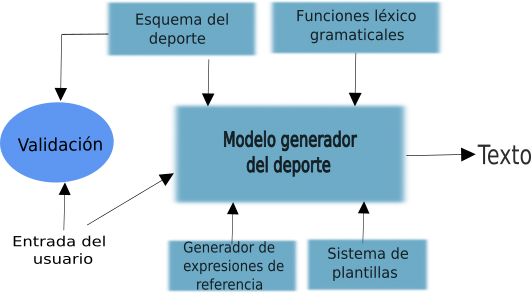
\includegraphics[scale=0.9]{Graphics/arquitecturatesisOKFINAL.png}
    \end{center}
    \caption{Arquitectura de modelo propuesta}
    \label{arquitecturadelmodeloOK}
\end{figure}

    La arquitectura general planteada se presenta en \ref{arquitecturadelmodeloOK} y constituye una 
adaptación de la propuesta de Aires \brackcite{aires2016automatic} que a su vez sigue un enfoque basado en la propuesta de Theune y col. \brackcite{theune2001data}. 
A diferencia de las mismas, el sistema propuesto no consume bases de conocimiento específicas, ya que busca adaptarse al hecho general del deporte a
abordar. Un sistema sencillo para generar expresiones de referencia se incluye con el objetivo de que los modelos generen un texto más fluido.

    Como se analizó en el capítulo anterior (\ref{chapter:state-of-the-art}), las tareas de los sistemas de generación de texto a partir de datos se pueden dividir en 
dos etapas: la referente al contenido a representar y su estructura (planificación del contenido) y la de realización lingüística. La planificación del contenido 
viene dada por la estructura extraída de los textos analizados. Para la etapa de realización, se propone un sistema basado en reglas y plantillas.

    \subsubsection{Realización lingüística}
 
    En la etapa de realización del texto se ven unificadas las tareas de carácter lingüístico tal y como se presentó en \ref{chapter:state-of-the-art}. 
En este proceso se determinan las palabras y expresiones con las que exponer el contenido seleccionado bajo la estructura definida. El enfoque basado en reglas 
y llenado de plantilla es de los más utilizados por el control que otorga sobre la producción del texto (\ref{subsection:lexicalizacion}). Tiene la ventaja de que 
se asegura la calidad estructural del texto producido, así como permite dotar de variabilidad a las salidas tal y como se discutió en el capítulo 
anterior (\ref{subsection:realizcion}).

    Las plantillas se utilizan dentro del modelo para conformar estructuras más complejas en forma de oraciones. Cada conjunto 
de plantillas dentro del sistema pertenece a una parte de la estructura del texto. Para cada contexto se conciben varias plantillas que brindan opciones para expresar la información relativa a una idea.

    Las plantillas pueden o no presentar ranuras para completar con información. Las ranuras se utilizan de la forma: \textit{$<$ dato $>$} donde 
\textit{dato} se sustituye por el valor de la variable que representa. Para dotar de facilidad al sistema a la hora de adaptarse a eventos de 
ambos géneros, se puede utilizar dentro de las plantillas expresiones como \textit{\$ expresión dependiente del género \$}, donde \textit{“expresión dependiente del género” }
se sustituye por su expresión de género correcta dentro del contexto a través de una de las funciones léxicas. El caracter “@” también se utiliza dentro de las plantillas 
para hacer distinciones de género. Por ejemplo en la frase: \textit{amb@s se golpearon}, el “@” se sustituye por “a” o por “o” en dependencia del género.
\\

\textbf{Funciones lingüísticas}\\

    Las funciones lingüísticas tienen el objetivo de mejorar la calidad del texto producido. Asimismo, buscan asegurar su correcta estructura gramatical. Una vez constituida una oración a partir de unificar plantillas de expresiones, una función se encarga de dotar de un 
formato a la misma. Se colocan las mayúsculas correspondientes al inicio, así como los puntos finales. Otra función se emplea para eliminar errores gramaticales o de 
estructura que se presentan durante la unión de las plantillas. Se eliminan los espacios en blanco múltiples, se corrigen los signos de puntuación así como los artículos 
repetidos y las construcciones mal formadas, como por ejemplo “de el”.

Otras funciones léxicas se utilizan para dar mayor fluidez al texto, como las que transforman expresiones numéricas en texto, por ejemplo, “3” por “tres”.
\\

\textbf{Generador de expresiones de referencia}\\

Las expresiones de referencia son las que permiten identificar unívocamente a una entidad dentro de un contexto \brackcite{reiter_dale_2000,Gatt2018SurveyOT}. 
Un sistema de expresiones de referencia debe determinar si la entidad a referenciar ha sido mencionada previamente, ya que existe una diferenciación entre la 
introducción de una entidad y su referencia tardía, tal y como se trató en el capítulo anterior (\ref{subsection:expreferencia}). A su vez, la expresión seleccionada 
para referirse a una entidad debe tener en cuenta el resto de entidades del dominio. Por ejemplo, en un evento donde “Alejandro González” y “Pedro González” sean 
protagonistas, la expresión “González” resulta ambigua. Se propone un generador de expresiones de referencia basado en los nombres propios de los integrantes del 
enfrentamiento, utilizando los apellidos como referencias tardías y el nombre completo en la introducción.



    



\chapter{Detalles de Implementación}\label{chapter:implementation}

%##1

Los modelos en build tienen que hacer todo el proceso de procesamiento de los datos, llenando tomados
las variables y estructuras que son necesarias para generar el texto en cada una de las etapas. Luego
en generate los modelos van en base a la representación interna de los datos, generando el texto de 
caa una de las piezas comunicativas.







%##2

Para poder trabajar más fácil con la propuesta, se proporcionó una interfaz gáfica. Esta interfaz es sencilla
 y se concibió utilizando el framework de python streamlit. Se da la opción a los usuarios de aportar
 datos en forma de archivos, ya sea a partir de definir la ruta local o cargando directamente el archivo.

 Para permitir  esta interacción se concibió una estructura intermedia para poder representar las tuplas
 de entrada en base a archivos json.  Cada tupla se concibe de la forma "id"

 donde cada valor representa el valor de la tupla............. en esa posición. Si no se proporciona uno de los 
 valores, esa posición se considera vacía. Ejemplo de representación se puede ver en imagen.

 Desde la primera interfaz se puede interactuar con el conjunto de datos de prueba que se concibieron
junto a la propuesta. Para ello hay que seleccionar el deporte deseado y uno entre los eventos de prueba.
El sistema mostrará el texto producido en pantalla, luego de presionar el botón "generar".


 




%##3

Para el llenado de la plantilla se utiliza la función select template, que a su vez emplea la función
fille template  y genre desambiguation.

La función  select template recibe el conjunto de posibles plantillas a emplear en la situación así como un 
diccionario de representación, donde las llaves constituyen las ranuras en las plantillas y los valores, el Valor
de ese dato en el contexto.

Como el sistema propuesto presenta cierto grado de sensibilidad ante la ausencia de datos, es posible
que haya plantillas en el conjunto para la que alguna de sus ranuras no tiene valor. Para esto, el algoritmo
selecciona automáticamente una plantilla del conjunto, si en el diccionario todas las ranuras tienen un valor 
correspondiente se selecciona, si no, se descarta y se repite el proceso. Siempre se garantiza que habrá
al menos una plantilla en el conjunto que funcione, porque presentará el subconjunto minimal de datos que
admite el sistema en ese contexto. La plantilla seleccionada se rellena utilizando el  método fill template
que sustituye las ranuras de la plantilla por el valor real.




\begin{figure}[!]
    \begin{center}
        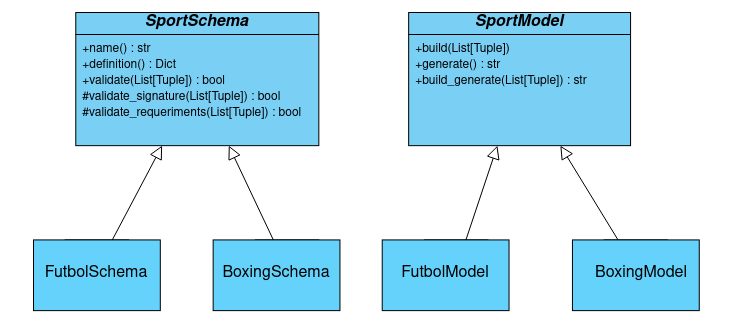
\includegraphics[width=\textwidth]{Graphics/classDef3.png}
    \end{center}
    \caption{Definición de las clases principales}
    \label{fig_classDef}
\end{figure}

\backmatter

\begin{conclusions}
    %Conclusiones   
    En el presente trabajo se definió la propuesta de un sistema para la 
generación de resúmenes de enfrentamientos deportivos, independiente de la fuente de datos del dominio, a
partir del análisis de características comunes del conjunto de los deportes de enfrentamiento.

Se presentó una propuesta de meta esquema general con el cual definir la estructura de entrada de
los datos al sistema y se validó que es posible, a partir de dicho esquema,  definir un esquema de representación individual por deporte. 
Se concibió una propuesta de diseño para los modelos de generación de un deporte en base a su esquema.
El fútbol y el boxeo demostraron ser muestras útiles para la validación del sistema, por ser disciplinas muy diferentes en cuanto a su naturaleza de 
ejecución y características.

    Se logró implementar un prototipo de sistemas con los modelos de generación para generar reportes basados en los eventos de estas dos
disciplinas deportivas. Los modelos, siguiendo un enfoque simple de reglas y plantillas, mostraron variabilidad en distintas ejecuciones frente a los 
mismos datos. A su vez, mostraron fidelidad en la información representada en la salida respecto a los datos de entrada y garantizaron la correcta estructura 
del texto producido. De esta forma, cumplieron con el requerimiento básico de los sistemas de generación de GLN funcionales.

    

\end{conclusions}



\begin{recomendations}
   % Recomendaciones

   A partir del análisis de los resultados obtenidos, se considera que el texto producido por los 
modelos presentados pudiera ser dotado de mayor fluidez. Agregar un mecanismo más potente
para la generaci\'on y selección de expresiones de referencia, pudiera contribuir
a esto, disminuyendo las repeticiones continuas del mismo nombre propio. Asimismo, la fluidez se puede mejorar definiendo reglas 
específicas para la agregación de eventos iguales consecutivos, o que presenten relación de causalidad.
También aumentar el número de plantillas para distintos tipos de expresiones, 
contribuiría a aumentar la variabilidad de los modelos.

Se recomienda evaluar la adaptabilidad de los esquemas propuestos a una diversidad de fuentes proveedoras de datos para comprobar su 
factibilidad en la práctica. Asimismo, se recomienda buscar una propuesta para la generación automática de las tuplas de 
conocimiento a partir de un esquema específico. 
 



\end{recomendations}

\include{BackMatter/Bibliography}

\end{document}